% ============================================================
% WCT Paper: INFORMS SERV Template Format
% When Front-Stage Innovation Overloads Back-Stage Workers
% Converted to INFORMS SERV (serv,dblanonrev) format
% ============================================================

\documentclass[serv,dblanonrev]{informs4}
\usepackage{eqndefns-left}
\RequirePackage{tgtermes}
\RequirePackage{newtxtext}
\RequirePackage{newtxmath}
\RequirePackage{bm}
\RequirePackage{endnotes}

\OneAndAHalfSpacedXII
\raggedbottom   % prevent vertical stretching on sparse pages

% Optional LaTeX Packages
\usepackage{tikz}
\usetikzlibrary{arrows.meta, positioning, calc, decorations.markings}
\usepackage{booktabs}

% Natbib setup for author-number style
\usepackage{natbib}
\bibpunct[, ]{(}{)}{,}{a}{}{,}%
\def\bibfont{\small}%
\def\bibsep{\smallskipamount}%
\def\bibhang{24pt}%
\def\newblock{\ }%
\def\BIBand{and}%

% Setup of the equation numbering system
\EquationsNumberedThrough

% Setup of theorem styles
\TheoremsNumberedThrough
\ECRepeatTheorems

% For new submissions, leave this number blank
\MANUSCRIPTNO{}

% Custom notation shortcuts
\newcommand{\Gp}{[G]^{+}}
\newcommand{\Gm}{[-G]^{+}}
\newcommand{\Keff}{K_{\mathrm{eff}}}

\begin{document}

\RUNAUTHOR{Authors suppressed}

\RUNTITLE{Front-Stage Innovation Overloads Back-Stage Workers}

\TITLE{When Front-Stage Innovation Overloads Back-Stage Workers:\
A Dynamic Model of Workforce, Capability, and Customer Trust
in Omnichannel Retail}

\ARTICLEAUTHORS{%
\AUTHOR{Authors suppressed for double-blind review}
\AFF{Affiliations suppressed, \EMAIL{suppressed}}
}

\ABSTRACT{%
Digital investment in omnichannel retail generates back-stage demand on
workers that standard dashboards cannot see, making workforce degradation
invisible until customer trust has already collapsed.
Front-stage automation amplifies operational complexity faster than
back-stage capacity can absorb it, creating a structural measurement gap:
technology returns and labour consequences appear on different ledgers,
and the workforce that determines whether technology delivers its designed
capability goes systematically underinvested.

We formalise this gap as a parsimonious dynamic model.
Three analytically characterised results follow.
A computable digitalisation ceiling exists beyond which additional
front-stage investment destroys customer lifetime value by overloading
back-stage workers; revenue metrics continue rising even as lifetime
value collapses.
The entire return to workforce investment flows through service capacity,
invisible to dashboards that treat payroll as a cost line.
The system is bistable: the neglected firm faces a safe rollout window
less than two-fifths the size of its investing peer.

These results supply two computable numbers absent from standard
dashboards: a digitalisation ceiling and a maximum safe rollout size.
Workforce investment is a structural requirement of digital strategy,
not a social concession.
}%

\KEYWORDS{omnichannel retail, workforce well-being, service capability, customer trust, system dynamics, people-centric operations}

\FUNDING{No external funding was received for this research.}

\maketitle

\section{Introduction}\label{sec:intro}

Omnichannel grocery retailers have invested heavily in digital capabilities in recent years \citep{hubner2021digitalization, bijmolt2021challenges}, enabling customers to build baskets across channels, reserve items for same-day collection, and track substitutions in real time. The business case for each investment is evaluated primarily through front-stage metrics: app engagement, order volume, and conversion rates. Yet as digital engagement has grown, retailers have encountered a structural asymmetry in how costs and returns are measured. Technology investment registers as successful in the domain where it is evaluated, while the back-stage workforce that must fulfil the digitally generated demand absorbs consequences that appear nowhere in the technology business case. \citet{corbett2024wellbeing} identifies this disconnect between digital investment and workforce well-being as a central open problem in operations management, observing that rapid changes in sectors such as warehousing and same-day delivery have created large numbers of newly stressful jobs whose well-being implications remain formally unmodelled.

The asymmetry is structural, not incidental. Omnichannel retailing places distinctive operational demands on back-stage workers (pickers, drivers, click-and-collect associates) because front-stage digital capabilities generate customer journeys that multiply handoff complexity far faster than order volume grows \citep{saghiri2017toward}. A basket built across three channels, fulfilled by a picker navigating real-time substitutions and customer approvals, represents qualitatively more cognitive and operational demand than its volume equivalent in a single-channel system. The empirical literature confirms the scale of these consequences. Workforce investment in retail generates returns that are both large and invisible to standard metrics: validated implementations find that the labour-to-revenue return is positive at every staffing level firms currently operate, yet most firms systematically understaff because dashboards track payroll as a cost percentage rather than as a revenue driver \citep{fisher2021staffing}. Responsible scheduling raises store productivity and sales, yet these gains register only in financial outcomes rather than in the operational metrics that govern staffing decisions \citep{kesavan2022doing}. The Good Jobs Strategy \citep{ton2014good} documents the same pattern from the management side: firms that invest in workforce capacity outperform on both operational and financial measures, but the causal chain runs through mechanisms (capability, service quality, and trust) that standard dashboards do not monitor.

What is missing from this body of evidence is a formal account of the mechanism. The empirical literature establishes that workforce investment pays off; it does not characterise \emph{when} additional front-stage investment begins to destroy rather than create value, \emph{how fast} a firm can scale digitalisation before the back-stage workforce is overwhelmed, or \emph{what dynamic relationship} connects technology investment, workforce well-being, and customer trust over time. These are not questions that regression analysis on historical data can answer: they require a model that treats workforce well-being and customer trust as co-evolving state variables responding to a controllable investment sequence. No formal model in the service quality-erosion tradition distinguishes between front-stage investments that generate demand and the back-stage workforce that fulfils it, nor treats customer trust as an endogenous dynamic that feeds back into the demand the workforce must absorb (see~\S\ref{sec:lit:erosion}).

The economic structure of the problem has a specific character that motivates the model architecture. Technology and workforce are not independent inputs to service capability but strategic complements in the sense of \citet{milgrom1990economics}: as automation handles more routine fulfilment tasks, the quality of residual human judgment at exception-handling, customer interaction, and quality verification becomes proportionally more consequential for overall output \citep{bainbridge1983ironies, kremer1993oring}. This complementarity implies that firms scaling digital investment without proportional workforce investment are not merely leaving money on the table but actively eroding the productivity of their existing technology base, because the workforce multiplier through which technology delivers service quality is declining. The damage accumulates invisibly: front-stage metrics measure the technology's demand-generation performance, which may continue to rise, while back-stage metrics for workforce effective capacity do not exist in most operational dashboards. By the time degradation becomes visible in customer satisfaction or retention data, the workforce tipping dynamic is already well advanced.

This paper formalises this economic structure as a parsimonious dynamic model. The central modelling innovation is the \emph{workforce capacity multiplier}: effective service capability is not the technology stock alone but the product of that stock and a workforce engagement index, so that technology and workforce are structural complements in the model's architecture. When front-stage demand grows faster than back-stage workforce capacity, a service gap opens that depletes workforce well-being, which reduces effective capability, which widens the gap further: a reinforcing deterioration that single-domain models cannot generate. Three formally characterised results follow. A \emph{Front-Stage Trap} (Theorem~\ref{thm:trap}): a computable digitalisation threshold exists beyond which additional front-stage investment reduces customer lifetime value by overloading back-stage workers, a cross-domain sign reversal impossible in models that do not separate the investing and absorbing domains. A \emph{Good Jobs Buffer} (Theorem~\ref{thm:buffer}): the return to workforce investment flows through a capacity-level channel that is dominant when the technology base is large and entirely invisible to dashboards that measure only operational sensing. A \emph{Burnout Cliff} (Theorem~\ref{thm:cliff}): the system exhibits bistability, and the maximum safe rollout speed is a workforce constraint: a firm that neglects its workforce faces a safe deployment window less than two-fifths the size of one that invests in its people.

A fourth result, Proposition~\ref{prop:complementarity}, establishes that the marginal value of workforce investment is increasing in digitalisation level. Since sustaining service quality at higher front-stage investment requires proportionally greater effective back-stage capability, the more digital the firm becomes, the more consequential the workforce multiplier becomes. Workforce investment is therefore not a social concession to employee well-being but a structural requirement of digital strategy, one that becomes more, not less, urgent as digitalisation deepens.


% ============================================================
% 2. LITERATURE REVIEW
% ============================================================

\section{Related Literature}\label{sec:lit}

This paper sits at the intersection of three research streams: service quality erosion in operations management, workforce-performance linkages in retail, and omnichannel capability management. We review each stream and identify the specific gaps the model addresses.

\subsection{Service Quality Erosion and Capability Dynamics}\label{sec:lit:erosion}

The foundational insight that service quality can erode endogenously under demand pressure originates with \citet{oliva2001cutting}, who use the system-dynamics framework of \citet{sterman2000business} to model reinforcing feedback loops in which workers cut corners and work overtime under demand pressure, producing death spirals. Their finding that workers are roughly twice as willing to cut corners as to work overtime grounds the overload-asymmetry parameter $\sigma$ in the present model. \citet{rahmandad2016capability} and \citet{repenning2001nobody} extend the logic to capability erosion and the invisibility of prevention effort, while extensions of the Oliva--Sterman (O-S) framework address e-commerce growth \citep{oliva2003limits} and regulatory compliance \citep{martinez2014drift}. At the empirical level, \citet{kc2009impact} show that sustained high workload increases service time and patient mortality, and \citet{corbett2024wellbeing} calls, in an OM Forum piece that explicitly sets the research agenda, for formal dynamic models that capture workforce well-being in operations, a call this paper directly addresses. None of these contributions introduces customer trust as a state variable, a front-/back-stage domain split, or a digital-scaling parameter.

\textbf{Gap 1.} Within the service quality-erosion and capability-erosion tradition, no formal model treats workforce well-being as a positive multiplier on service capability; all treat it as a degradation channel. \textbf{Gap 2.} No Oliva--Sterman extension adds customer trust, a front-/back-stage split, or digital scaling.


\subsection{Workforce Investment and Retail Performance}\label{sec:lit:workforce}

A substantial empirical literature documents the link between workforce practices and retail performance. \citet{ton2014good} identifies four operational choices (offer less, standardise and empower, cross-train, and operate with slack) that constitute the ``Good Jobs Strategy.'' The causal link from workforce investment to financial performance has been established through rigorous studies: \citet{kesavan2022doing} show in a field experiment at Gap Inc.\ that stable, predictable scheduling raised labour productivity by 5.1\% and median sales by 3.3\%, while \citet{fisher2021staffing} demonstrate through validated implementation that profit-maximising staffing is considerably higher than prevailing practice. \citet{dube2020minimum} confirm at the labour-economics level that employment conditions and firm-level wage practices shape worker performance and retention. The conceptual mechanism connecting these findings is the \emph{service profit chain} \citep{heskett1994putting}: internal service quality drives employee engagement, which drives customer loyalty and profitability. To the best of our knowledge, the service profit chain has not been formalised as a dynamic model with explicit feedback loops and boundary conditions; the present model provides this formalisation. The Job Demands-Resources model \citep{bakker2007job, demerouti2001job} provides the micro-foundation for how workforce well-being responds to operational conditions: demands deplete well-being at an accelerated rate under overload, while resources and direct investment restore it, with diminishing returns as the workforce approaches full capacity. Two features of this evidence motivate the model's dynamic structure. First, the Job Demands-Resources (JD-R) literature establishes a systematic asymmetry: the depletion rate under overload significantly exceeds the recovery rate under equivalent surplus. Second, \citet{mas2009peers} find that productivity responses to working conditions scale with current engagement level: the more engaged the workforce, the more sensitive performance is to changes in conditions in either direction. These two features together (asymmetric overload response and engagement-scaled sensitivity) underpin the workforce dynamics formalised in \S\ref{sec:model:dynamics}.

\textbf{Gap 3.} No dynamic model formalises the Good Jobs Strategy or the service profit chain with explicit feedback loops, analytical equilibria, and computable boundary conditions specifying \emph{when} workforce investment dominates capability investment.


\subsection{Omnichannel Capability and Cross-Domain Demand}\label{sec:lit:omni}

The omnichannel retailing literature documents the complexity of managing integrated service delivery across channels \citep{bijmolt2021challenges}. \citet{hubner2021digitalization} show that digitalisation creates considerable challenges for retail logistics, with fulfilment complexity scaling super-linearly as channel combinations increase; \citet{saghiri2017toward}, \citet{bell2018inventory}, and \citet{acimovic2015fulfillment} provide evidence consistent with this super-linearity. The technology-workforce interaction has received limited formal treatment in the omnichannel operations literature. \citet{bainbridge1983ironies} observed that automation shifts the operator's role toward exception handling, requiring \emph{higher} skill and engagement. A related mechanism appears in O-ring automation theory \citep{gans2026oring}: as tasks are automated, the quality of residual human tasks becomes more consequential for overall output. \citet{milgrom1990economics} and \citet{aral2012three} establish the formal conditions and empirical evidence for technology--workforce strategic complementarity: the return to investing in one resource increases when the other is also developed. This motivates the model's central structural assumption that the marginal value of workforce engagement rises with the size of the technology base, an assumption formalised and tested in \S\ref{sec:model:stocks}.

\textbf{Gap 4.} No model formalises the cross-domain mechanism by which front-stage digital investment creates super-linear demand on back-stage workers. \textbf{Gap 5.} The digitalisation-workforce cross-partial has not been derived for service operations.

Taken together, these gaps leave firms without any formal instrument for the two decisions that matter most: how much to invest in the workforce relative to front-stage technology, and how fast to scale digitalisation without triggering an irreversible service collapse. Existing models cannot generate the computable thresholds (a digitalisation ceiling and a maximum safe rollout size) that would make these decisions tractable.

\medskip
\noindent Table~\ref{tab:gaps} summarises the five gaps and the model's response to each; no prior work addresses all five simultaneously, and the single structural innovation (effective capability as the product of technology and workforce engagement) generates each contribution as a direct consequence.

\begin{table}
\TABLE
{Literature gaps and model contributions.\label{tab:gaps}}
{\begin{tabular}{@{}p{0.40\textwidth}p{0.22\textwidth}p{0.27\textwidth}@{}}
\toprule
\textbf{Gap} & \textbf{Closest prior work} & \textbf{This paper} \\
\midrule
1.\ No model treats $W$ as a positive capability multiplier &
    \citet{oliva2001cutting}: $W$ as degradation only &
    Effective capability as the product of technology and workforce engagement \\[6pt]
2.\ No Oliva--Sterman extension adds trust, domain split, or digital scaling &
    \citet{oliva2001cutting}; \citet{martinez2014drift} &
    Customer trust as a co-evolving state; front/back domain split; digital scaling \\[6pt]
3.\ Good Jobs Strategy / service profit chain (SPC) unformalised &
    \citet{ton2014good}; \citet{heskett1994putting}: empirical only &
    Dynamic formalisation with analytical equilibria and boundary conditions \\[6pt]
4.\ No cross-domain front-to-back overload model &
    \citet{saghiri2017toward}: conceptual only &
    Super-linear back-stage demand as a function of digital depth and customer trust \\[6pt]
5.\ Digitalisation-workforce cross-partial not derived for services &
    No direct service prior; see also \citet{gans2026oring} (O-ring) &
    Formally derived: the return to workforce investment rises with the technology base \\
\bottomrule
\end{tabular}}{}\end{table}

\section{Model}\label{sec:model}

Sections~\ref{sec:model:stocks}--\ref{sec:model:loops} formalise the workforce capacity multiplier introduced in \S\ref{sec:intro}. The front-stage digitalisation level $F > 0$ is treated as an exogenous managerial control: it sets the complexity and volume of customer-facing digital features, and thereby determines the demand placed on the back-stage operation. The model traces the dynamic consequences of choosing $F$ for the three co-evolving back-stage state variables and, through them, for customer lifetime value (CLV). Each of the eight free parameters has a single, distinct role with a clean kill condition (Table~\ref{tab:params}): setting it to its neutral value eliminates exactly one mechanism, allowing the model to nest single-domain benchmarks as special cases.

\subsection{Stocks and Effective Capability}\label{sec:model:stocks}

Three state variables evolve jointly: $K(t) > 0$, the back-stage technology stock (installed infrastructure, warehouse management systems, and process standardisation); $W(t) \in (0,1)$, an index of workforce well-being (engagement, energy, and cognitive capacity among pickers, drivers, and click-and-collect associates); and $T(t) \in (0,1)$, customer trust (the customer base's aggregate confidence that the retailer will deliver reliably). All three are dimensionless and normalised to their natural operating ranges. Throughout, starred variables ($K^*$, $W^*$, $T^*$) denote steady-state equilibrium values; the pre-shock (baseline) digitalisation level is written $F_0$; and $\Delta F$ denotes an upgrade step, the increase in $F$ from $F_0$.

The central structural innovation is the \emph{effective capability}. The economic premise is that a warehouse management system, routing algorithm, or substitution-handling process can only deliver its designed performance if the workforce operating it has the capacity to do so: a burned-out picker cannot execute a real-time exception protocol effectively regardless of how sophisticated the supporting technology is. This means effective capability is not the technology stock alone but its product with a workforce engagement multiplier:
\begin{align}\label{eq:Keff}
    \Keff(t) &\;=\; K(t) \cdot h\bigl(W(t)\bigr), \notag\\
    h(W) &= (1-p) + pW, \quad p \in (0,1).
\end{align}
Effective capability is the product of the technology stock and a workforce capacity multiplier $h(W)$. The multiplier ranges from $h(0) = 1-p$ (at zero well-being, the workforce delivers only the irreducible, automation-driven fraction $1-p$ of the technology's designed potential) to $h(1) = 1$ (a fully engaged workforce realises the technology's full design capacity). The cross-partial
\begin{equation}\label{eq:cross_partial}
    \frac{\partial^2 \Keff}{\partial K\, \partial W} \;=\; p \;>\; 0
\end{equation}
is strictly positive for all $p > 0$, establishing technology and workforce as complements in the \citet{milgrom1990economics} sense.

The parameter $p$ governs complementarity: $p = 0$ decouples workforce from capability; $p = 1$ makes the operation fully labour-intensive. The baseline $p = 0.5$, motivated by capital-skill complementarity evidence \citep{krusell2000capital}, represents a moderate starting point; estimation is discussed in \S\ref{sec:disc:limits}. All three theorems hold qualitatively for any $p \in (0,1)$.


\subsection{Demand and the Service Gap}\label{sec:model:demand}

Customer demand on back-stage operations is
\begin{equation}\label{eq:demand}
    D(T, F) \;=\; (1 + aT) \cdot F^b,
\end{equation}
where $a > 0$ is the trust-demand coupling and $b > 1$ is the front-stage amplification exponent. The trust-demand coupling reflects the established finding that customer trust drives spending consolidation and order frequency \citep{sirdeshmukh2002consumer, mcknight2002developing}. The super-linearity $b > 1$ captures the well-documented increase in back-stage fulfilment complexity as front-stage channel breadth grows: as shown in \S\ref{sec:lit:omni}, \citet{bell2018inventory} and \citet{acimovic2015fulfillment} document patterns consistent with fulfilment error rates and demand-capacity mismatches rising faster than linearly with channel combinations. We set $b = 1.3$ as an illustrative, structurally conservative baseline motivated by this literature; the Front-Stage Trap requires only $b > 1$, and all three theorems hold qualitatively across $b \in [1.1, 2.0]$ (EC Table~EC.3).

The \emph{service gap} measures the shortfall between demand and effective capability:
\begin{equation}\label{eq:gap}
    G(t) \;=\; D\bigl(T(t),\, F\bigr) \;-\; K(t) \cdot h\bigl(W(t)\bigr).
\end{equation}
When $G > 0$ (overload), customers experience failures. When $G < 0$ (surplus), service runs reliably. We write $\Gp = \max(G,0)$ and $\Gm = \max(-G,0)$ for the positive and negative parts.


\subsection{Dynamics}\label{sec:model:dynamics}

The feedback loops in \S\ref{sec:model:loops} are built from the three ordinary differential equations (ODEs) introduced below, which translate each economic mechanism into a rate equation. All rate parameters carry units of months$^{-1}$; each ODE is piecewise-smooth, activating different terms in the overload regime ($G > 0$, so $[G]^+ = G$, $[-G]^+ = 0$) and the surplus regime ($G < 0$, so $[G]^+ = 0$, $[-G]^+ = -G$).

\paragraph{Capability.}
The technology stock evolves as
\begin{equation}\label{eq:dK}
    \frac{dK}{dt} \;=\; r\,\Gp\, W \;-\; \delta\, K \;+\; u,
\end{equation}
where $r > 0$ is the sensing-adaptation rate, $\delta > 0$ is the depreciation rate, and $u \geq 0$ is direct back-stage investment. The sensing term $r\,\Gp\, W$ captures organisational learning from service failures: the product structure requires both a gap to detect ($\Gp > 0$) \emph{and} workforce capacity to act on it ($W > 0$). When workers are burned out, failure signals go unheeded. This formulation is grounded in \citet{tucker2007operational}, who shows that frontline employees are the primary mechanism through which operational failures translate into system improvement. The term activates only under overload ($G > 0$), reflecting the well-documented asymmetry in organisational learning: firms learn more from failures than from routine success \citep{repenning2001nobody, rahmandad2016capability}. The multiplicative $W$ structure rather than an additive correction is supported by \citet{argote1990learning}, who show that capability accumulation scales with the workforce knowledge stock, and by \citet{mas2009peers}, who find that productivity responses are amplified by current engagement levels.

\paragraph{Workforce well-being.}
Well-being rises when the operation runs with surplus capacity (the workforce is not overwhelmed and has room to recover) and when the firm directly invests in people through scheduling, training, and operational support. It falls through natural decay; engagement requires maintenance even under ordinary conditions. Under overload, depletion accelerates at a rate empirically higher than the recovery rate under equivalent surplus. Formally:
\begin{equation}\label{eq:dW}
    \frac{dW}{dt} = \bigl(\Gm + f\bigr)(1 - W) - \bigl(\mu + \sigma\,\Gp\bigr) W.
\end{equation}
Two grouped terms ensure $W(t) \in [0,1]$ for all $t \geq 0$ whenever $W(0) \in [0,1]$: the first term drives $W$ upward and vanishes at $W = 1$; the second drives $W$ downward and vanishes at $W = 0$. \emph{Recovery and investment} ($(\Gm + f)(1 - W)$): capability surplus and direct workforce investment both raise well-being, with diminishing returns as $W$ approaches full capacity, consistent with the resources buffer in the JD-R model \citep{bakker2007job}. \citet{kesavan2022doing} provide causal evidence: responsible scheduling at Gap Inc.\ raised productivity by 5.1\%. \emph{Depletion} ($({\mu + \sigma\,\Gp})\,W$): natural decay ($\mu$) and overload-amplified erosion ($\sigma\,\Gp$) both deplete well-being, with the overload effect scaled by $\sigma > 1$. The value $\sigma = 2.0$ is set as a magnitude comparator consistent with \citeauthor{oliva2001cutting}'s (\citeyear{oliva2001cutting}) finding that workers are roughly twice as willing to cut corners as to work overtime; this is a comparator from a service-industry study rather than a direct estimate of the depletion-rate asymmetry in a burnout ODE, and all three theorems hold qualitatively for any $\sigma > 1$ (EC Table~EC.3).

\paragraph{Customer trust.}
Customer trust builds slowly through consistently reliable service and erodes faster when that reliability fails, a well-documented asymmetry in service industries where negative experiences are weighted more heavily than positive ones. Trust also decays naturally over time in the absence of positive reinforcement, reflecting the gradual shifting of customer expectations and the competing claims of rival channels. Formally:
\begin{equation}\label{eq:dT}
    \frac{dT}{dt} \;=\; \beta\,\Gm\,(1 - T) \;-\; \eta\,\beta\,\Gp\, T \;-\; \lambda\, T,
\end{equation}
where $\beta > 0$ is the trust-update rate, $\eta > 1$ is the erosion asymmetry, and $\lambda > 0$ is natural trust decay. The asymmetric structure reflects the robust finding that negative service experiences damage trust more than positive experiences build it \citep{baumeister2001bad, mittal1998asymmetric}. We set $\eta = 2.0$, consistent with the asymmetric coefficients reported by \citet{sirdeshmukh2002consumer} for frontline employee operational benevolence in retail (approximately 2.5:1 depletion-to-enhancement ratio). The three equations above constitute a piecewise-smooth system; the remark below establishes its analytical properties before the loop architecture is presented.


\begin{remark}[Piecewise-Smooth Dynamics]\label{rem:pwsmooth}
The system (\ref{eq:dK})--(\ref{eq:dT}) is piecewise-smooth, with a non-smooth gradient at the switching manifold $\mathcal{M} = \{G = 0\}$. Existence and uniqueness of solutions follow from Filippov's (\citeyear{filippov1988differential}) framework, provided trajectories cross $\mathcal{M}$ transversally; numerical verification at both equilibria confirms this under baseline parameters. Crucially, the implicit function theorem arguments underpinning the analytical results are applied at surplus equilibria where $G^* = -S^* < 0$, so differentiability is guaranteed by the smooth structure of the ODE within $\{G < 0\}$; smoothing robustness is verified in EC~\S EC.1.8.
\end{remark}

\subsection{State-Space Invariance and Empirical Mapping}\label{sec:model:invariance}

The state space $K > 0$, $W \in [0,1]$, $T \in [0,1]$ is forward-invariant for all $t \geq 0$; the verification via directional derivatives at each boundary is given in EC~\S EC.1.1.

Observable field proxies include: app feature index for front-stage capability ($F$), employee engagement composite for workforce well-being ($W$), net promoter score for customer trust ($T$), and on-time fulfilment shortfall for the service gap ($G$). Parameter calibration details are in EC~\S EC.4.


\subsection{Feedback-Loop Architecture}\label{sec:model:loops}

Figure~\ref{fig:loops} shows the causal-loop architecture of the three ODEs, using the conventions of \citet{sterman2000business}. The diagram contains four feedback loops, each traceable from the state-variable arrows.

\textbf{Loop R1} ($T \to D \to G \to T$, reinforcing): customer trust raises demand, demand changes the service gap, and the gap feeds back to trust. In the surplus regime ($G < 0$), this loop is self-sustaining: higher trust generates demand that the capable operation absorbs, preserving trust.

\textbf{Loop R2} ($G \to W \to K_{\mathrm{eff}} \to G$, reinforcing): overload depletes workforce well-being, lower well-being reduces effective capability through the multiplier $h(W)$, and reduced capability widens the gap further. This is the deterioration loop behind the Front-Stage Trap.

\textbf{Loop R3} ($W \to K_{\mathrm{eff}} \to G \to W$, reinforcing): workforce well-being contributes to effective capability; when overload erodes capability and widens the gap, workforce depletion accelerates. This is the escalation loop behind the Burnout Cliff.

\textbf{Loop B1} ($G \to K \to K_{\mathrm{eff}} \to G$, balancing): overload triggers sensing investment in the technology stock, which raises effective capability and closes the gap. This is the corrective loop that stabilises the surplus equilibrium when overload is moderate.

Loops R2 and R3, created by the capacity multiplier $h(W)$, have no counterpart in prior quality-erosion models; they are the structural mechanisms by which workforce degradation becomes self-reinforcing. Note that R2 traces how overload propagates from the gap to the workforce; R3 traces how capability degradation escalates from the workforce back through the gap.

\newsavebox{\cldbox}
\savebox{\cldbox}{%
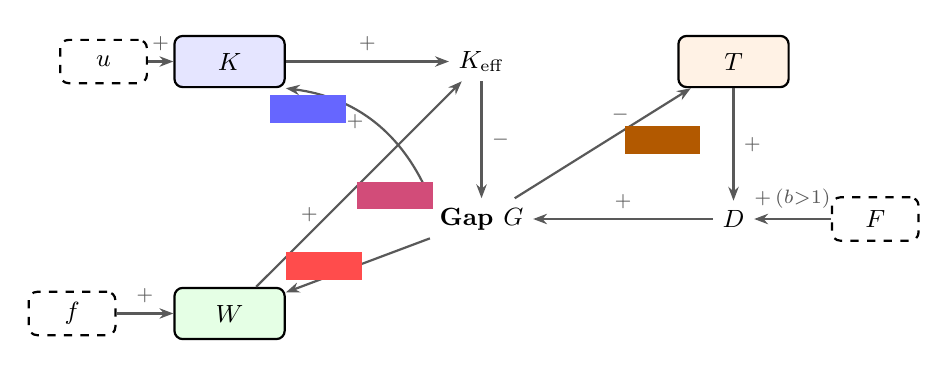
\begin{tikzpicture}[
    node distance=2.0cm and 2.8cm,
    stock/.style={rectangle, draw, thick, rounded corners=3pt, minimum width=1.4cm, minimum height=0.65cm, font=\small\bfseries},
    param/.style={rectangle, draw, dashed, thick, rounded corners=3pt, minimum width=1.1cm, minimum height=0.55cm, font=\small},
    aux/.style={font=\small},
    arr/.style={-{Stealth[length=5pt]}, thick, color=black!65},
    looplabel/.style={font=\scriptsize\bfseries, fill=white, inner sep=1.5pt}
]
    % Layout: K top-left, T top-right, W bottom-centre, Gap middle, D right
    \node[stock, fill=blue!10] (K) at (0, 3.2) {$K$};
    \node[aux] (Keff) at (3.2, 3.2) {$K_{\mathrm{eff}}$};
    \node[aux, font=\small\bfseries] (G) at (3.2, 1.2) {Gap $G$};
    \node[stock, fill=orange!10] (T) at (6.4, 3.2) {$T$};
    \node[aux] (D) at (6.4, 1.2) {$D$};
    \node[stock, fill=green!10] (W) at (0, 0) {$W$};

    % Controls placed to avoid visual overlap with state-variable arrows
    \node[param] (F) at (8.2, 1.2) {$F$};
    \node[param] (f) at (-2.0, 0) {$f$};
    \node[param] (u) at (-1.6, 3.2) {$u$};

    % Arrows
    \draw[arr] (K) -- node[above, font=\scriptsize]{$+$} (Keff);
    \draw[arr] (W) -- node[left, font=\scriptsize, pos=0.35]{$+$} (Keff);
    \draw[arr] (Keff) -- node[right, font=\scriptsize]{$-$} (G);
    \draw[arr] (G) -- node[left, font=\scriptsize, pos=0.4]{$-$} (W);
    \draw[arr] (T) -- node[right, font=\scriptsize]{$+$} (D);
    \draw[arr] (D) -- node[above, font=\scriptsize]{$+$} (G);
    \draw[arr] (G) -- node[above, font=\scriptsize, pos=0.6]{$-$} (T);
    % F->D arrow routes via a short horizontal segment to avoid passing through T
    \draw[arr] (F) -- node[above, font=\scriptsize]{$+\,(b{>}1)$} (D);
    \draw[arr] (G.north west) to[bend right=30] node[left, font=\scriptsize]{$+$} (K.south east);
    \draw[arr] (f) -- node[above, font=\scriptsize]{$+$} (W);
    \draw[arr] (u) -- node[above, font=\scriptsize]{$+$} (K);

    % Loop labels: positioned at loop centroids with polarity signs
    \node[looplabel, color=orange!70!black] at (5.5, 2.2) {\textsf{R1} $(+)$};
    \node[looplabel, color=purple!70] at (2.1, 1.5) {\textsf{R2} $(+)$};
    \node[looplabel, color=red!70] at (1.2, 0.6) {\textsf{R3} $(+)$};
    \node[looplabel, color=blue!60] at (1.0, 2.6) {\textsf{B1} $(-)$};
\end{tikzpicture}}

\begin{figure}
\FIGURE
{\usebox{\cldbox}}
{Causal-loop architecture of the WCT model. Solid boxes are state variables ($K$, $W$, $T$); dashed boxes are exogenous controls ($F$, $f$, $u$). Arrow signs indicate direction of effect ($+$ same direction, $-$ opposite direction); loop polarity is shown in parentheses beside each label ($+$ reinforcing, $-$ balancing). $F$ is positioned adjacent to $D$ to clarify that the $F \to D$ link is direct (with super-linear scaling $b > 1$) and distinct from the $F \to T$ path, which does not exist in the model. Loop R1 ($T \to D \to G \to T$, reinforcing) is the trust--demand self-reinforcement loop; its effective polarity depends on the sign of $G$. Loop R2 ($G \to W \to K_{\mathrm{eff}} \to G$, reinforcing) is the workforce-capacity deterioration loop behind the Front-Stage Trap. Loop R3 ($W \to K_{\mathrm{eff}} \to G \to W$, reinforcing) is the workforce-capability escalation loop behind the Burnout Cliff. Loop B1 ($G \to K \to K_{\mathrm{eff}} \to G$, balancing) is the sensing-investment corrective loop that stabilises the surplus equilibrium. Loops R2 and R3 are created by the capacity multiplier $h(W)$ and do not exist in single-domain models.\label{fig:loops}}
{R2, R3 are novel; neither exists in Oliva--Sterman (2001).}
\end{figure}


\subsection{Parameters and Special Cases}\label{sec:model:params}

Table~\ref{tab:params} summarises all parameters. Two control variables complete the model: $u \geq 0$ (capability investment) and $f \geq 0$ (workforce investment). The model recovers the core dynamics of \citet{oliva2001cutting} when $p = 0$ and $a = 0$ (see EC \S EC.2 for the structural mapping), and reduces to a Solow-type capital-accumulation equation when $p = 0$, $a = 0$, and $r = 0$.

\begin{table}
\TABLE
{Model parameters, baseline values, and kill conditions.\label{tab:params}}
{{\setlength{\tabcolsep}{3pt}\small
\begin{tabular}{@{}cp{0.26\textwidth}cccp{0.19\textwidth}p{0.22\textwidth}@{}}
\toprule
\# & Parameter & Baseline & Timescale & Kill & Mechanism killed & Empirical anchor \\
\midrule
1 & $b$ (demand super-linearity) & 1.3 & -- & $b{=}1$ & Front-Stage Trap & Bell et al.\ (2018); Acimovic \& Graves (2015) \\
2 & $a$ (trust-demand coupling) & 0.4 & -- & $a{=}0$ & Demand feedback & McKnight et al.\ (2002); Sirdeshmukh et al.\ (2002) \\
3 & $p$ (workforce complementarity) & 0.5 & -- & $p{=}0$ & Capacity multiplier & Krusell et al.\ (2000) \\
4 & $\sigma$ (overload asymmetry) & 2.0 & -- & $\sigma{=}1$ & Tipping point & \citet{oliva2001cutting}; \citet{bakker2007job}$^\dagger$ \\
5 & $\eta$ (erosion asymmetry) & 2.0 & -- & $\eta{=}1$ & Trust asymmetry & Sirdeshmukh et al.\ (2002) \\
6 & $r$ (sensing-adaptation) & 0.4 & $\tau_{r} \approx 1.7$ mo & $r{=}0$ & Self-correction dies & Tucker (2007); Argote \& Epple (1990) \\
7 & $\delta$ (depreciation) & 0.03 & $\tau_{\delta} \approx 23$ mo & -- & -- & Illustrative (EC \S EC.4) \\
8 & $\beta$ (trust-update rate) & 0.12 & $\tau_{\beta} \approx 5.8$ mo & $\beta{\to}0$ & Trust frozen & Illustrative (EC \S EC.4) \\
\addlinespace
+ & $\mu$ (natural $W$ decay) & 0.05 & $\tau_{\mu} \approx 14$ mo & $\mu{=}0$ & $W$ experiential only & Demerouti et al.\ (2001); Dub\'e et al.\ (2020) \\
+ & $\lambda$ (natural $T$ decay) & 0.025 & $\tau_{\lambda} \approx 28$ mo & $\lambda{=}0$ & $T$ experiential only & Illustrative (EC \S EC.4) \\
\bottomrule
\end{tabular}
}}{All time units are months. Timescales for rate parameters are $\ln(2)/\theta$ (half-life). The model has eight free parameters (rows~1--8); the two supplementary rows ($\mu$, $\lambda$) govern natural decay and all three theorems hold for any $\mu,\lambda>0$. Parameters labelled ``Illustrative'' are calibrated within empirically informed ranges; see EC~\S EC.4. Dimensionless parameters (rows 1--5) do not carry timescale units. $^\dagger$The 2:1 ratio is a magnitude comparator from a professional-services context, not a direct structural estimate for retail; see \S\ref{sec:model:dynamics} for qualification. Empirical anchors in the final column motivate the qualitative structure and plausibility of each parameter value; they are not direct structural estimates. Direct estimation of $b$ and $p$ from retailer panel data is discussed as the primary empirical extension in \S\ref{sec:disc:limits}.}\end{table}
\section{Analytical Results}\label{sec:analysis}

Having established the model's architecture, we now show that the structural separation between the domain that invests in digital capabilities and the domain that absorbs the consequences generates three phenomena that no single-domain model can produce. We derive four formal results. Theorems~\ref{thm:trap}--\ref{thm:cliff} characterise the three counter-intuitive phenomena the model produces; Proposition~\ref{prop:complementarity} establishes the digitalisation-workforce complementarity. Full proofs are in the Electronic Companion (\S EC.1); here we provide proof sketches that convey the economic intuition.

\subsection{Equilibrium Structure}\label{sec:analysis:eq}

The model generates two distinct long-run outcomes, each recognisable to retail operations practitioners. In the first, the back-stage operation runs with sufficient capacity to absorb the digital demand placed on it: the workforce is healthy, customers experience reliable service, trust builds, and the firm settles into a self-reinforcing high-performance state. Formally, this is the \emph{surplus equilibrium}, the system's preferred resting point when effective capability exceeds demand. In the second, demand has overwhelmed capability: the workforce is depleted, service quality has deteriorated, and customers have largely withdrawn their trust. The firm is trapped at a \emph{low-trust attractor} from which exit requires a structural intervention, not merely a temporary reduction in digital ambition.

The technical characterisation of these two states is as follows. The surplus equilibrium exists for all $F < F_{\mathrm{crit}}$ and is unique under Condition C2 (EC Lemma~2, \S EC.1.2). When effective capability exceeds demand, define the operational surplus $S^* \equiv K^*h(W^*) - D(T^*,F) \geq 0$ as the excess of effective capability over demand at equilibrium. Equilibrium trust is an increasing function of $S^*$, saturating toward one as surplus grows: $T^* = \beta S^* / (\beta S^* + \lambda)$. Equilibrium well-being is similarly increasing in surplus and investment: $W^* = (S^* + f) / (S^* + f + \mu)$. The capability stock settles at $K^* = u/\delta$, determined entirely by the investment-depreciation balance. Full algebraic derivations are in EC~\S EC.1.2. Both $T^*$ and $W^*$ are increasing in $S^*$, so any improvement in effective capability propagates into higher trust and well-being at the equilibrium, creating the reinforcing dynamics that underpin the Good Jobs Buffer.

The low-trust attractor is reached whenever demand persistently overwhelms capability. With $T^* \approx 0$, demand collapses to its digitalisation-driven floor and the workforce settles at a low but strictly positive well-being level, held above zero by the workforce investment rate $f$. Effective capability at this attractor falls short of demand, maintaining a persistent residual gap. The attractor exists whenever $F^b > (u/\delta)\,h(W^*_{\mathrm{low}})$ and is locally stable (EC Remark~1).

\paragraph{Maintained conditions.}
The formal results in the following subsections hold under four regularity conditions. These are not strong restrictions; they amount to requiring that the surplus equilibrium exists, is unique, and that the low-trust attractor is also present. All four conditions are verified analytically or numerically across the empirically relevant parameter space (see EC Remark~3 for details): (C1)~surplus equilibrium existence ($F < F_{\mathrm{crit}}$; analytic via the Intermediate Value Theorem, IVT); (C2)~uniqueness (analytic under a single-crossing sufficient condition, C2-SC: $\beta(f{+}\mu)<\lambda$, which holds for all $f\in[0,0.10]$ regardless of $b$, $p$, $\sigma$; EC~\S EC.1.2); (C3)~regularity ($\Phi'(S^*) < 0$; consequence of C1--C2); and (C4)~low-trust attractor existence ($F^b > (u/\delta)\,h(W^*_{\mathrm{low}})$; numeric Jacobian verification).

\begin{remark}[Analytical Transparency]\label{rem:transparency}
Because the results below combine fully analytic derivations with computational verification, the table classifies each result by its evidentiary basis. Tier~A results hold for all parameter values satisfying the stated conditions; Tier~B results hold analytically subject to the maintained regularity conditions (C1)--(C4); Tier~C results are computationally verified over the studied parameter space but not proved globally. The table may be consulted alongside each theorem as a reference.
\smallskip

\noindent
{\small\renewcommand{\arraystretch}{0.92}%
\begin{tabular}{@{}p{0.38\textwidth}p{0.08\textwidth}p{0.42\textwidth}@{}}
\toprule
\textbf{Result} & \textbf{Tier} & \textbf{Basis} \\
\midrule
Thm~1(i): equilibrium existence/nonexistence & A & Analytic (IVT + $\Phi(0)$ sign) \\
Thm~1(ii): trajectories bounded & A & Analytic (Gronwall; Lemma~3) \\
Thm~1(ii): wide-basin convergence & C & Numerical grid, $K_0=K^*$ slice \\
Lemma~2 (uniqueness of $S^*$) & B & Analytic under C2-SC ($\beta(f{+}\mu)<\lambda$; holds throughout parameter space; EC~\S EC.1.2) \\
Thm~2: $\partial\,\mathrm{CLV}^*/\partial f > 0$ (sign) & B & IFT chain; GE feedback correction sign analytic \\
Thm~2: GE feedback magnitude (${\approx}0.09$) & C & Confirmed across 100 configurations \\
Thm~3(i): $\Delta F_{\mathrm{collapse}}$ threshold & A & Direct from Thm~1 \\
Thm~3(i): convergence from pre-shock IC & C & Numerical; basin-dependent \\
Prop~1 cross-partial & A & Analytic ($\Keff = Kh(W)$) \\
Prop~1 $F_{\max}(W)$ boundary formula & A & Exact at $S^*\to 0$ \\
Prop~1 $F_{\max}(W)$ interior upper bound & B & Analytic sign; ${\approx}8\%$ correction numeric \\
Corollary~5, Case~1 & B & Thm~1 + Thm~2 directly \\
Corollary~5, Case~2 near $B_{\min}$ & B & Continuity from Case~1 (IFT; EC~\S EC.1.7) \\
Corollary~5, Case~2 interior & C & Computational; $c_F/c_f\in[0.5,5]$ \\
\bottomrule
\end{tabular}}
\end{remark}


\subsection{Theorem 1: The Front-Stage Trap}\label{sec:analysis:trap}

What happens to a retailer that keeps expanding its digital feature set? The intuitive answer is that each new capability generates incremental revenue. The model reveals a more complex dynamic. When each additional layer of digital investment generates back-stage fulfilment demand faster than proportional revenue (because fulfilment complexity grows super-linearly with channel breadth), a digitalisation level exists beyond which additional front-stage investment reduces rather than raises the quality of service the back-stage operation can deliver. At that point, adding digital features actively destroys customer lifetime value by overloading the workforce. This cross-domain sign reversal is the Front-Stage Trap.

\begin{theorem}[Front-Stage Trap]\label{thm:trap}
Suppose $b > 1$ and $p > 0$. Define the digitalisation threshold
\begin{equation}\label{eq:Fcrit}
    F_{\mathrm{crit}} \;=\; \Bigl(\frac{u}{\delta}\cdot\Bigl[(1-p)+p\,\frac{f}{f+\mu}\Bigr]\Bigr)^{1/b},
\end{equation}
which depends only on exogenous parameters $(u,\delta,p,f,\mu,b)$ and equals $K^*h(f/(f+\mu))^{1/b}$, the capacity multiplier evaluated at the boundary workforce level. Then:
\begin{enumerate}
    \item[(i)] For $F < F_{\mathrm{crit}}$, the surplus equilibrium (unique under C2; Lemma~2, EC~\S EC.1.2) exists with $T^* > 0$ and $\mathrm{CLV}^* > \mathrm{CLV}_{\mathrm{low}}$ (the CLV at the low-trust attractor).
    \item[(ii)] For $F \geq F_{\mathrm{crit}}$, no surplus equilibrium exists. All forward trajectories remain in a bounded compact set (Lemma~3, EC~\S EC.1.2), and the low-trust attractor is locally stable (EC Remark~1).
\end{enumerate}
The threshold $F_{\mathrm{crit}}$ is decreasing in $p$ and increasing in $f$: the Trap binds earlier when workforce-technology coupling is strong, and is relaxed by workforce investment.
\end{theorem}

\begin{remark}[Computability of $F_{\mathrm{crit}}$]\label{rem:Fcrit_implicit}
The implicit balance condition $K^*h(W^*)=(1+aT^*)F^b+S^*$ rearranges to $F=(K^*h(W^*)/(1+aT^*))^{1/b}$, but this is self-referential since $W^*$ and $T^*$ depend on $F$. Equation~(\ref{eq:Fcrit}) is the computable form: it evaluates $h$ and the demand term at the boundary $S^*\to 0$ where $T^*\to 0$, yielding a closed-form threshold.
\end{remark}

\noindent\textbf{Numerical result (convergence beyond $F_{\mathrm{crit}}$).}
While local stability of the low-trust attractor is established analytically (EC Remark~1), the claim that trajectories starting from a broad range of initial conditions converge to this attractor is verified computationally. Numerical integration across all initial conditions on the $K_0 = K^*$ slice of the simulation grid ($W_0 \in [0.08, 0.82]$, $F \in [0.70, 1.95]$) confirms convergence to the low-trust attractor with $T^*\approx 0$ and $\mathrm{CLV}\approx\mathrm{CLV}_{\mathrm{low}}$ for $F \geq F_{\mathrm{crit}}$; EC~\S EC.4.2 confirms the same qualitative structure for varied $K_0$.
\medskip

\noindent\textit{Proof sketch.}
The surplus equilibrium requires $\Phi(0) > 0$ (where $\Phi(S) \equiv K^*h(W^*(S)) - D(T^*(S),F) - S$ is the surplus residual; full construction in EC~\S EC.1.2), which holds if and only if $F < F_{\mathrm{crit}}$. At $F = F_{\mathrm{crit}}$, the surplus $S^* = 0$ and the equilibrium ceases to exist. For $F > F_{\mathrm{crit}}$, $G > 0$, activating overload depletion of $W$ through Eq.~(\ref{eq:dW}), which reduces $h(W)$, which further widens $G$ through Loop R2. The reinforcing dynamics drive the system toward the low-trust attractor. That trajectories remain bounded for all $t$ follows from Lemma~3 (EC~\S EC.1.2): under overload, $\dot{K} \leq C(F) - \delta K$ where $C(F) = r(1+a)F^b + u$ is a demand-capacity bound, giving $K(t)\leq\max(K_0,\,C(F)/\delta)$ by Gronwall's lemma; together with $W,T\in[0,1]$ by construction, the state space is forward-invariant and compact. Full proof in EC~\S EC.1.3. \Halmos

\medskip
This cross-domain CLV sign reversal, namely that additional front-stage investment beyond $F_{\mathrm{crit}}$ lowers CLV, requires $b > 1$: with linear demand ($b = 1$), the equilibrium-existence threshold still exists, but there is no sign reversal in CLV because demand does not grow faster than capacity. The condition $p > 0$ is required for $F_{\mathrm{crit}}$ to be workforce-contingent (increasing in $f$); at $p = 0$ the threshold reduces to $(u/\delta)^{1/b}$ and no longer responds to workforce investment. The result is structurally impossible in single-domain models such as \citet{oliva2001cutting} or \citet{rahmandad2016capability}, which cannot generate a cross-domain demand-capacity mismatch of this form. Analytically, the surplus equilibrium (high CLV) exists for all $F < F_{\mathrm{crit}} \approx 1.11$; for $F \geq F_{\mathrm{crit}}$, the only stable state is the low-trust attractor (CLV $\approx 400$). Figure~\ref{fig:bifurcation} maps this regime structure across the joint space of initial workforce well-being $W_0$ and digitalisation level $F$: green cells converge to the surplus attractor; red cells converge to the low-trust attractor. The basin boundary aligns with the analytic $F_{\mathrm{crit}}$ threshold and confirms the bistability underlying Theorem~\ref{thm:cliff}. At the calibrated baseline, $F_{\mathrm{crit}} \approx 1.11$ corresponds to roughly a 40\% increase in digital feature complexity above the starting level ($F_0 = 0.80$), consistent with the transition from basic click-and-collect to real-time substitution management requiring per-order picker adaptation.

\begin{figure}
\FIGURE
% Production filename: fig2_basin_map.png
{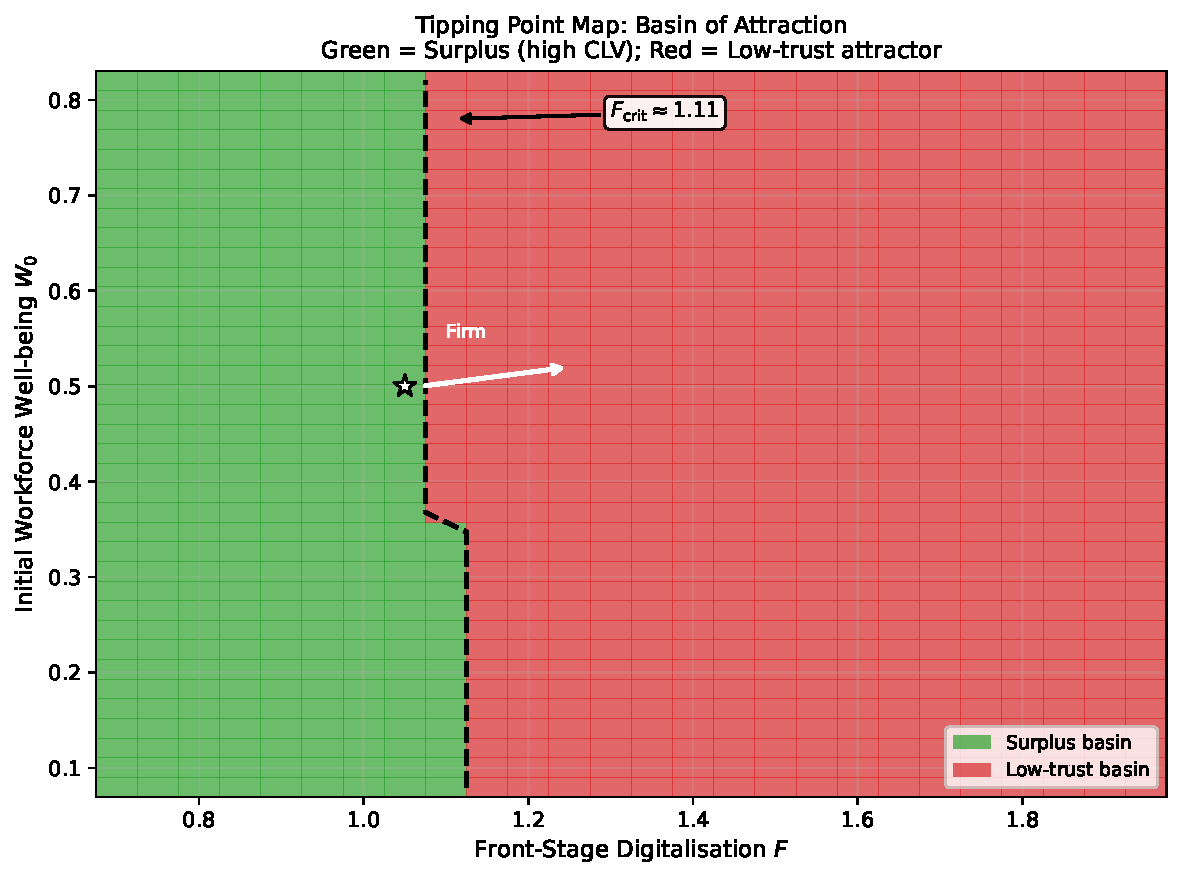
\includegraphics[width=0.75\textwidth]{fig2_basin_map.pdf}}
{Basin-of-attraction map: the Front-Stage Trap as regime structure. Green cells converge to the surplus attractor (high CLV) for $F < F_{\mathrm{crit}} \approx 1.11$; red cells converge to the low-trust attractor (CLV $\approx 400$) for $F \geq F_{\mathrm{crit}}$. The basin boundary is consistent with the analytic $F_{\mathrm{crit}}$ threshold; its $W_0$-dependence reflects trajectory dynamics beyond the scalar threshold, consistent with the bistability of Theorem~\ref{thm:cliff}. Doubled-grid validation (73$\times$51 trajectories; EC~\S EC.4.2) confirms boundary stability. Simulation methodology in EC~\S EC.4.2.\label{fig:bifurcation}}
{}
\end{figure}


\subsection{Theorem 2: The Good Jobs Buffer}\label{sec:analysis:buffer}

The empirical literature documents that workforce investment pays off, but the mechanism remains poorly understood. Why does the return to workforce investment appear to grow with firm size and digital sophistication? The model provides a precise answer: the payoff to workforce investment flows through the capacity-multiplier channel. A more engaged workforce raises effective capability not just by contributing additional effort but by unlocking more of the technology's designed potential. This multiplicative channel is invisible to dashboards that measure workforce investment as a cost line and technology investment as a revenue driver; the two returns are attributed to different domains, so the productivity of their interaction goes unmeasured. Theorem 2 characterises this channel exactly.

\begin{theorem}[Good Jobs Buffer]\label{thm:buffer}
Suppose $p > 0$ and the surplus equilibrium exists and is stable (Conditions C1--C4, i.e., the surplus equilibrium exists, is unique, and the low-trust attractor is present; Remark~\ref{rem:transparency}). Workforce investment $f$ raises steady-state CLV through a multiplicative capacity-level channel:
\begin{equation}\label{eq:buffer}
    \frac{\partial\,\mathrm{CLV}^*}{\partial f} \;>\; 0 \qquad \text{for all } f \geq 0.
\end{equation}
The return decomposes into a direct capacity effect and an indirect trust effect:
\begin{align*}
    \frac{\partial\,\mathrm{CLV}^*}{\partial f}
    &= \underbrace{\frac{\partial\,\mathrm{CLV}}{\partial T^*}
       \cdot \frac{\partial T^*}{\partial S^*}
       \cdot K^* \cdot p}_{\text{direct: } h(W) \text{ raises } \Keff}
       \cdot \frac{\partial W^*}{\partial f} \\
    &\quad +\;
    \underbrace{\text{higher-order terms via sensing}}_{\text{indirect: } W \text{ in } r\Gp W}.
\end{align*}
\end{theorem}

\noindent\textit{Proof sketch.}
Since $W^* = (S^* + f)/(S^* + f + \mu)$ at the surplus equilibrium, differentiating gives $\partial W^*/\partial f = \mu/(S^* + f + \mu)^2 > 0$: workforce investment raises steady-state well-being. Higher $W^*$ raises $h(W^*) = (1-p) + pW^*$, which increases $\Keff = K^* \cdot h(W^*)$, which widens the surplus $S^*$, which raises $T^* = \beta S^*/(\beta S^* + \lambda)$, which raises CLV. Each link is strictly positive: $\partial h/\partial W = p > 0$, $\partial S/\partial h = K^* > 0$, $\partial T^*/\partial S^* > 0$, $\partial\,\mathrm{CLV}/\partial T^* > 0$. The chain-rule product is therefore positive, and diminishing returns follow from the concavity of $W^*$ in $f$. Full proof in EC~\S EC.1.4. \Halmos

\medskip
The practical significance of this channel decomposition is confirmed in \S\ref{sec:sim:fig4_hidden}: the $p{=}0$ counterfactual shows that disabling the workforce multiplier leaves equilibrium CLV exactly invariant to workforce spending, confirming that the entire CLV return flows through service capacity rather than the operational sensing channel. Conventional workforce return-on-investment (ROI) calculations, which measure only the sensing channel, therefore structurally underestimate the financial return to workforce investment. The error is not merely one of magnitude but of mechanism: standard dashboards can, in principle, observe and attribute the sensing-channel return (improved failure detection, faster capability accumulation), yet the capacity-multiplier channel — through which workforce engagement unlocks the technology's designed potential — is invisible to any metric that records technology and workforce returns in separate ledgers. A firm evaluating workforce ROI through standard methods would reach the conclusion that investment is low-priority using correct data and sound arithmetic, and still be wrong.

\subsection{Theorem 3: The Burnout Cliff}\label{sec:analysis:cliff}

How fast can a retailer safely scale its digital operations? The standard answer focuses on technology capacity: rollout speed is limited by infrastructure readiness. The model reveals a different constraint. When a firm upgrades its digital features, it places a step-increase in demand on the back-stage workforce. If this demand increment exceeds what the current workforce can absorb without tipping into depletion, the system collapses permanently, even if the technology itself is fully functional. The critical insight is that the maximum safe upgrade size is determined not by the technology stock but by the current level of workforce investment. A firm that has neglected its workforce faces a much narrower safe rollout window than one that has invested in it. This is the Burnout Cliff: a hard deployment speed limit set by workforce headroom, not infrastructure capacity.

\begin{theorem}[Burnout Cliff]\label{thm:cliff}
Suppose $\sigma > 1$, $p > 0$, and $F_0 < F_{\mathrm{crit}}$ (a surplus equilibrium exists at $F_0$). Under these conditions the system is bistable in a neighbourhood of $F_{\mathrm{crit}}$. Consider a firm at the surplus equilibrium that implements a step increase in $F$ from $F_0$ to $F_0 + \Delta F$. Two thresholds govern the outcome:
\begin{enumerate}
    \item[(i)] \emph{Permanent-collapse onset.} For $\Delta F \geq \Delta F_{\mathrm{collapse}}$, no surplus equilibrium exists at the post-upgrade level. The low-trust attractor is the only locally stable state (EC Remark~1); convergence to it is confirmed numerically across the studied initial conditions.
    \begin{align*}
       \Delta F_{\mathrm{collapse}} &= F_{\mathrm{crit}} - F_0 \\
         &= \Bigl(\frac{u}{\delta}\bigl[(1\!-\!p)+p\tfrac{f}{f+\mu}\bigr]\Bigr)^{\!1/b} \!-\, F_0.
    \end{align*}
    For $\Delta F < \Delta F_{\mathrm{collapse}}$, a new surplus equilibrium exists at the post-upgrade level. Whether a given trajectory reaches this equilibrium depends on its initial condition relative to the basin boundary (Figure~\ref{fig:bifurcation}); numerical verification confirms convergence from the pre-shock equilibrium initial condition across the parameter configurations studied (EC~\S EC.4.2).
    \item[(ii)] \emph{Instantaneous-overload diagnostic.} A second, larger threshold marks the boundary above which demand turns positive at $t=0^+$:
    \begin{equation}\label{eq:DFrapid}
        \Delta F_{\mathrm{rapid}} \;=\; \frac{S_0}{b\cdot F_0^{b-1}\cdot(1+aT^*)},
    \end{equation}
    where $S_0 = K^*h(W^*) - D(T^*,F_0)$ is the pre-upgrade surplus. Because $\Delta F_{\mathrm{rapid}} > \Delta F_{\mathrm{collapse}}$ (at baseline: 0.40 vs.\ 0.31), a firm in the zone $\Delta F \in [\Delta F_{\mathrm{collapse}},\Delta F_{\mathrm{rapid}})$ collapses permanently but through a \emph{slow} trajectory ($G$ negative at $t=0^+$, surplus eroded gradually). For $\Delta F \geq \Delta F_{\mathrm{rapid}}$, $G$ turns positive immediately and the system enters a rapid self-reinforcing collapse to the low-trust attractor.
\end{enumerate}
The safe zone is $\Delta F < \Delta F_{\mathrm{collapse}}$; $\Delta F_{\mathrm{rapid}}$ is a deployment-speed diagnostic, not a safety threshold.
\end{theorem}

\noindent\textit{Proof sketch.}
Part (i) follows directly from Theorem~\ref{thm:trap}: for $F_0+\Delta F \geq F_{\mathrm{crit}}$, no surplus equilibrium exists; for $\Delta F < \Delta F_{\mathrm{collapse}}$, a new surplus equilibrium exists at $F_0+\Delta F$, and numerical verification confirms that trajectories originating at the pre-shock surplus equilibrium converge to this new surplus equilibrium across the parameter configurations studied (EC~\S EC.4.2). For Part~(ii), setting the first-order demand increment $\Delta D \approx (1+aT^*)\,b\,F_0^{b-1}\,\Delta F$ equal to the pre-upgrade surplus $S_0$ gives $\Delta F_{\mathrm{rapid}}$. Under overload the workforce tipping threshold (the $W$ level below which depletion rate exceeds recovery rate) is $W_{\mathrm{tip}} = f/(f + \mu + \sigma G_0^+)$; when $\Delta F < \Delta F_{\mathrm{rapid}}$, $G_0^+ = 0$ at $t_0^+$ and the system crosses $W_{\mathrm{tip}}$ through a slow transient, consistent with the slow-collapse zone. Full proof in EC \S EC.1.5. \Halmos

\medskip
From Part~(i), workforce investment $f$ raises $F_{\mathrm{crit}}$ and enlarges the safe upgrade zone: two firms with identical technology but different $f$ face different $\Delta F_{\mathrm{collapse}}$. Once a firm crosses the collapse threshold, Loop~R3 ($W \to K_{\mathrm{eff}} \to G \to W$) amplifies the deterioration: workforce depletion reduces effective capability, which widens the gap, which further depletes the workforce. The practical implication is directional: before each deployment phase, the firm should compute $\Delta F_{\mathrm{collapse}} = F_{\mathrm{crit}}(f) - F_0$ and treat it as a hard ceiling on planned upgrade size, independent of infrastructure readiness. The size of this ceiling is set entirely by the workforce investment rate $f$.


\subsection{Proposition 1: Digitalisation-Workforce Complementarity}\label{sec:analysis:comp}

\begin{proposition}[Digitalisation-Workforce Complementarity]\label{prop:complementarity}
The marginal value of workforce improvement is strictly increasing in the technology base:
\begin{align}\label{eq:complementarity}
    \frac{\partial \Keff}{\partial W} &= p \cdot K, \\
    \frac{\partial^2 \Keff}{\partial W\,\partial K} &= p > 0. \notag
\end{align}
Since maintaining surplus at higher $F$ requires higher effective capability $\Keff$ (that is, either higher $K^*$ through increased $u$, or higher $h(W^*)$ through increased $f$), the equilibrium return to workforce investment increases with digitalisation level.

Equivalently, workforce well-being determines the maximum sustainable digitalisation level. At the regime boundary ($S^* \to 0$), the equilibrium trust approaches zero ($T^* \to 0$; see Lemma~2, EC~\S EC.1.2), so:
\begin{equation}\label{eq:Fmax}
    F_{\max}(W) \;=\; \bigl(K^* \cdot h(W)\bigr)^{1/b},
\end{equation}
which is strictly increasing in $W$ for $p > 0$. The full implicit differentiation accounting for $T^*(W,F)$ dependence at interior equilibria (where $S^* > 0$) yields a correction term of order $O(aS^*)$ that vanishes as $S^* \to 0$; the formula (\ref{eq:Fmax}) is therefore exact at the boundary and an upper bound on $F_{\max}$ in the interior: trust-elevated demand means true safe capacity is somewhat lower than this formula implies (EC \S EC.1.6).
\end{proposition}

\noindent\textit{Proof.} The cross-partial follows directly from $\Keff = K[(1-p)+pW]$. The $F_{\max}$ formula identifies $F_{\mathrm{crit}}$ at $S^*\to 0$, where $T^*\to 0$, giving $(K^*h(W))^{1/b}$, strictly increasing in $W$ since $h'(W)=p>0$; with the full $T^*(W,F)$ correction this is exact at the boundary and an upper bound in the interior (EC~\S EC.1.6). \Halmos

\medskip
This comparative-statics result connects to and extends the O-ring automation insight of \citet{gans2026oring}: front-stage automation (higher $F$) requires a larger back-stage technology base ($K$), which raises the marginal value of the workforce operating that technology ($pK$). Workforce neglect becomes proportionally more costly as the technology base grows. Figure~\ref{fig:complementarity} illustrates equation~(\ref{eq:Fmax}) directly: the gap between a stressed firm ($W = 0.30$, $F_{\max} \approx 1.063$) and a healthy one ($W = 0.70$, $F_{\max} \approx 1.307$) is 23\%, arising entirely from workforce investment with no change to the technology stock.

\begin{figure}
\FIGURE
% Production filename: fig3_complementarity.png
{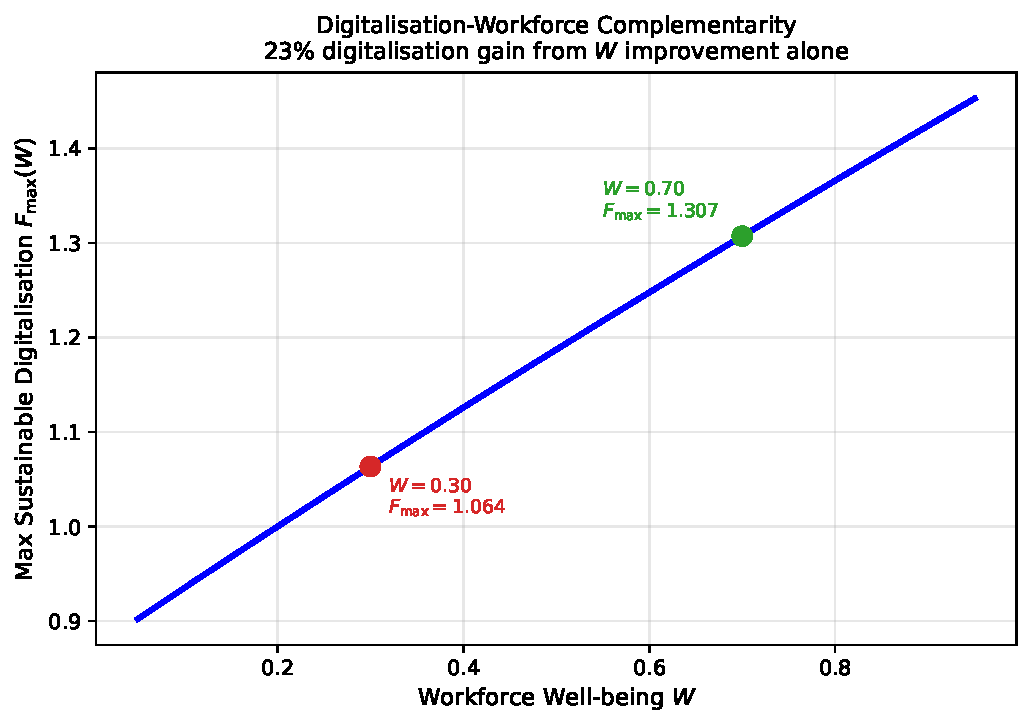
\includegraphics[width=0.75\textwidth]{fig3_complementarity.pdf}}
{Digitalisation-workforce complementarity. Workforce well-being determines the maximum sustainable digitalisation level $F_{\max}(W) = (K^* h(W))^{1/b}$: the healthy firm (green, $W=0.70$) sustains 23\% higher $F$ than the stressed firm (red, $W=0.30$). The boundary slope $\partial F_{\max}/\partial W = (p/b)(K^*)^{1/b}[h(W)]^{1/b-1}$ confirms that workforce matters more as the firm scales digitally.\label{fig:complementarity}}
{}
\end{figure}

\medskip
The budget corollary directly answers the allocation question practitioners face most immediately: given a fixed investment budget, should the firm prioritise front-stage technology or back-stage workforce? Let $c_F > 0$ and $c_f > 0$ denote the per-unit costs of front-stage and workforce investment respectively, and $B_{\min} \equiv c_F \cdot F_{\mathrm{crit}}$ the budget at which the all-$F$ corner exactly reaches the Trap threshold. Under a budget constraint $c_F F + c_f f \leq B$, the all-$F$ corner is strictly dominated when $B \geq c_F F_{\mathrm{crit}}$ (Case~1): Theorem~\ref{thm:trap} implies $\partial\,\mathrm{CLV}/\partial F \leq 0$ while Theorem~\ref{thm:buffer} guarantees $\partial\,\mathrm{CLV}^*/\partial f > 0$, so reallocating any marginal dollar to $f$ produces a strict gain. For smaller budgets (Case~2: $B < c_F F_{\mathrm{crit}}$), strict dominance of $f$ holds analytically in a neighbourhood of $B_{\min}$ by continuity from Case~1 (per-dollar returns are continuous in $F$ via the IFT) and computationally across $c_F/c_f \in [0.5,5]$ throughout the studied range. The CLV-maximising allocation satisfies $f^* > 0$ analytically for Case~1 and for the near-$B_{\min}$ sub-case of Case~2; the interior of Case~2 is established computationally across the studied parameter range, not analytically (proof and scope in EC~\S EC.1.7).

\section{Computational Study}\label{sec:simulation}

We illustrate the analytical results through calibrated simulations using the baseline parameters in Table~\ref{tab:params}. CLV follows \citet{gupta2004valuing}: $\mathrm{CLV} = w(T)/(1-\rho(T))$, where $\rho(T)$ is an annual retention probability and $w(T)$ an annualised per-customer margin, with $\rho(T) = 0.80 + 0.18T$ and $w(T) = 80(1 + 0.25\max(T-0.15,0))$. The endpoints $\rho(0)=0.80$ and $\rho(1)=0.98$ fall within the 70--90\% annual range in \citet{gupta2004valuing}; \pounds 80 is an illustrative annual margin for UK omnichannel grocery. All analytical results hold for any CLV increasing in trust (calibration in EC~\S EC.4.3). All three qualitative phenomena are robust across $b \in [1.1, 2.0]$, $\sigma \in [1.0, 3.0]$, and $p \in [0.25, 0.75]$ (EC Table~EC.3).

\subsection{The Hidden Cost of App Innovation (Figure~\ref{fig:hidden_cost})}\label{sec:sim:fig4_hidden}

Three deployment strategies are compared, designed to span the analytically critical threshold identified in Theorem~\ref{thm:trap}. Scenarios~A and~C deliberately target a front-stage level above $F_{\mathrm{crit}} \approx 1.11$, crossing into the Front-Stage Trap; Scenario~B targets a level below the threshold, remaining in the surplus regime. The CLV divergence across scenarios therefore reflects both a timing effect and a threshold effect, consistent with Theorem~\ref{thm:trap}. All three begin from the same starting state $(K_0, W_0, T_0) = (1.60, 0.55, 0.50)$ with $F_0 = 0.80$ and back-stage investment $u = 0.05$. Scenario~A ramps aggressively to $F_{\mathrm{end}} = 1.15$ with no workforce investment; Scenario~B ramps moderately to $F_{\mathrm{end}} = 1.05$ with concurrent workforce support ($f=0.06$); Scenario~C pre-invests in workforce ($f=0.10$, months 1--12, after which $f$ returns to zero as the front-stage ramp begins) before ramping to $F_{\mathrm{end}} = 1.15$.

Figure~\ref{fig:hidden_cost} shows that all three scenarios appear profitable in app revenue KPIs (panel~a), yet CLV diverges sharply (panel~b): by month~24, Scenario~C sustains CLV approximately 40\% above Scenario~A. Panel~(a) plots the front-stage demand-volume index $F \cdot D(T(t), F(t))$ (proportional to revenue under constant margin; the product of digitalisation level and the demand it generates), which shows sustained net growth across all three scenarios regardless of back-stage state; this is the metric visible to the team that made the investment decision, and its upward trend masks the divergence unfolding in panels~(c) and (d), showing $W$ and $T$ respectively. Workforce collapse precedes trust collapse, confirming the cross-domain cost invisible in the technology business case and the Front-Stage Trap mechanism of Theorem~\ref{thm:trap}: front-stage metrics register the investment as successful precisely because the back-stage consequences appear on a different ledger. The capacity-multiplier mechanism of Theorem~\ref{thm:buffer} is confirmed by a $p{=}0$ counterfactual: disabling the multiplier leaves equilibrium CLV invariant to workforce spending at any $f$ (EC Table~EC.4, indirect-channel share $<1\%$), confirming the entire CLV return flows through service capacity rather than operational sensing.

\begin{figure}
\FIGURE
% Production filename: fig4_hidden_cost.png
{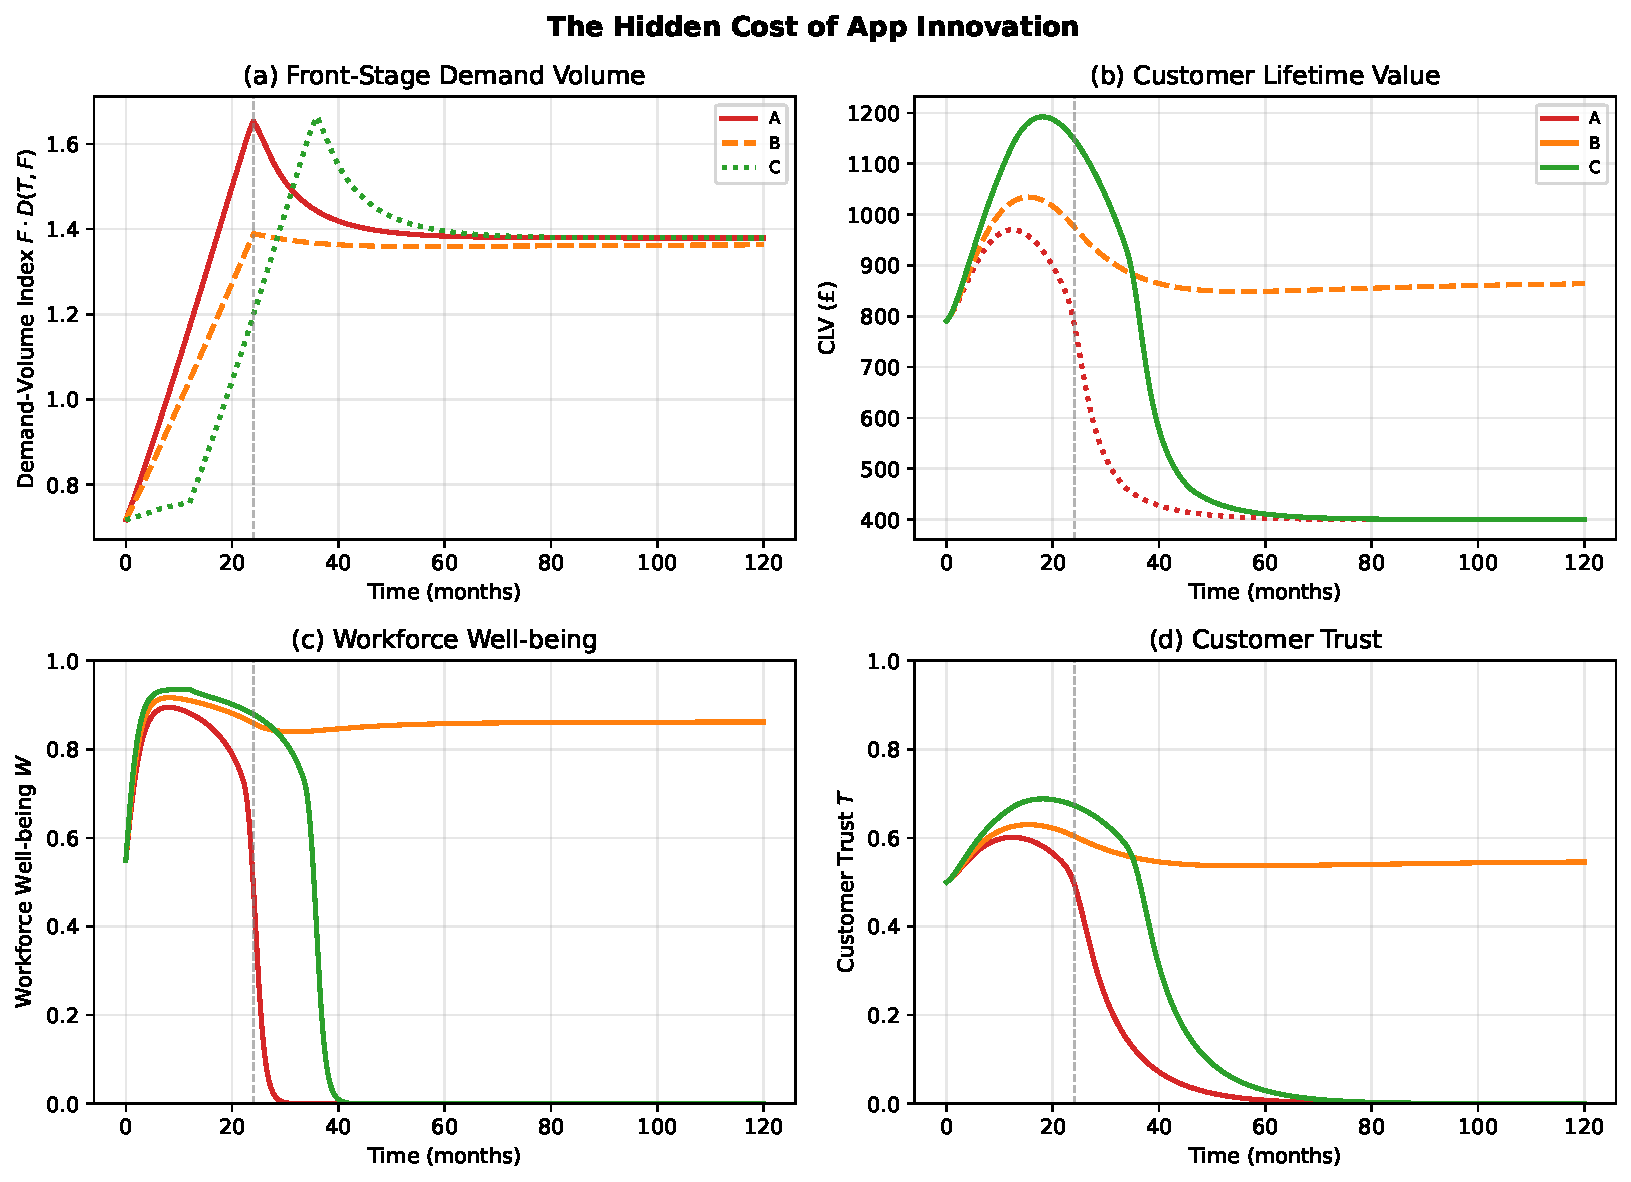
\includegraphics[width=\textwidth]{fig4_hidden_cost.pdf}}
{The hidden cost of app innovation. Three deployment strategies from the same starting state, differing in both front-stage target ($F_{\mathrm{end}} = 1.15$ for Scenarios A and C; $F_{\mathrm{end}} = 1.05$ for Scenario B) and workforce investment timing (none, concurrent, or pre-emptive). Panel~(a) plots the front-stage demand-volume index $F \cdot D(T(t),F(t))$, which rises for all three scenarios and provides no signal of divergence. CLV (panel~b) diverges sharply by month~24 as workforce collapse (panel~c) precedes trust collapse (panel~d) in the no-investment scenario.\label{fig:hidden_cost}}
{}
\end{figure}


\subsection{Basin-of-Attraction Structure}\label{sec:sim:fig2}

The bistability established in Theorem~\ref{thm:cliff} implies a basin-of-attraction boundary separating firms that recover from a deployment shock from those that collapse to the low-trust attractor. Figure~\ref{fig:bifurcation} maps this boundary across the joint space of $W_0$ and $F$: firms below the boundary (green) converge to high CLV; those above (red) converge to the low-trust attractor. The map answers a question retail technology teams rarely ask directly: given where we are today, how much runway do we have before a deployment shock becomes irreversible? Firms in the upper-left of the map (high digitalisation, low workforce well-being) have essentially no safe zone remaining; firms in the lower-right (moderate digitalisation, healthy workforce) retain large margins. The basin boundary is consistent with $\Delta F_{\mathrm{collapse}}$ and shifts rightward as $W_0$ increases, consistent with the prediction that workforce well-being directly enlarges the safe operating region. Crucially, a firm currently operating near the basin boundary can increase its safety margin not by reducing technology investment but by increasing workforce investment $f$: higher $f$ shifts $F_{\mathrm{crit}}$ rightward, moving the firm further from the collapse boundary without touching the technology stock. Doubled-grid validation (EC~\S EC.4.2) confirms the boundary position is numerically stable.

\subsection{The Burnout Cliff (Figure~\ref{fig:cliff})}\label{sec:sim:fig5}

We sweep upgrade size $\Delta F \in [0, 0.60]$ for three workforce-investment scenarios: neglected ($f=0.01$), baseline ($f=0.03$), and invested ($f=0.10$). Each scenario starts from its own surplus equilibrium $(K^*, W^*, T^*)$ at $F_0 = 0.80$. The equilibrium workforce well-being rises from $W^* = 0.928$ at $f=0.01$ to $W^* = 0.937$ at $f=0.10$; the analytically critical difference is the shift in $F_{\mathrm{crit}}(f)$, driven by the boundary workforce level $f/(f+\mu)$ (which spans 0.17 to 0.67 across scenarios) rather than the operating $W^*$. This shifts $F_{\mathrm{crit}}(f)$ from $0.98$ to $1.29$, widening $\Delta F_{\mathrm{collapse}}$ from $0.18$ to $0.49$. Separately, the Good Jobs Buffer (Theorem~\ref{thm:buffer}) is confirmed analytically via the workforce ROI decomposition (EC Table~EC.6): at $F = 0.85$, raising $f$ from $0.01$ to $0.10$ raises equilibrium CLV from approximately \pounds 1{,}323 to \pounds 1{,}334 (a \pounds 11 gain), while the $p{=}0$ counterfactual shows exactly zero response across the same $f$ range. Although the absolute gain is modest at $F = 0.85$ (well within the surplus regime), the structural result is exact: 100\% of the return flows through the capacity-multiplier channel, and the sensing channel contributes nothing, confirming Theorem~\ref{thm:buffer}.

Figure~\ref{fig:cliff} shows the three CLV curves as a function of $\Delta F$. Each curve is normalised to $\mathrm{base} = 100$ at $\Delta F = 0$ to allow comparison of cliff locations. Vertical markers show $\Delta F_{\mathrm{collapse}}$ (permanent onset, dotted) and $\Delta F_{\mathrm{rapid}}$ (instantaneous overload, dashed). For the neglected-workforce scenario ($f=0.01$), the safe zone collapses to $\Delta F < 0.18$; for the invested scenario ($f=0.10$), the cliff recedes beyond $\Delta F = 0.49$. The slow-collapse zone between $\Delta F_{\mathrm{collapse}}$ and $\Delta F_{\mathrm{rapid}}$ is the region where dashboards report continued revenue growth while the underlying trust trajectory has already turned negative: this is the diagnostic blind spot identified in the paper's opening argument, now quantified as a zone width of approximately 0.09 digitalisation units at the baseline. Notably, this blind spot is a feature of under-investment: for the well-investing firm ($f=0.10$), the slow-collapse zone disappears entirely because $\Delta F_{\mathrm{rapid}} < \Delta F_{\mathrm{collapse}}$ (established formally in EC~\S EC.1.5). High workforce investment does not merely widen the safe zone; it also converts the collapse regime from gradual invisible deterioration into a sharp, observable threshold that a firm can plan around. Collapse detection and simulation details are in EC~\S EC.4.2.

\begin{figure}
\FIGURE
% Production filename: fig5_burnout_cliff.png
{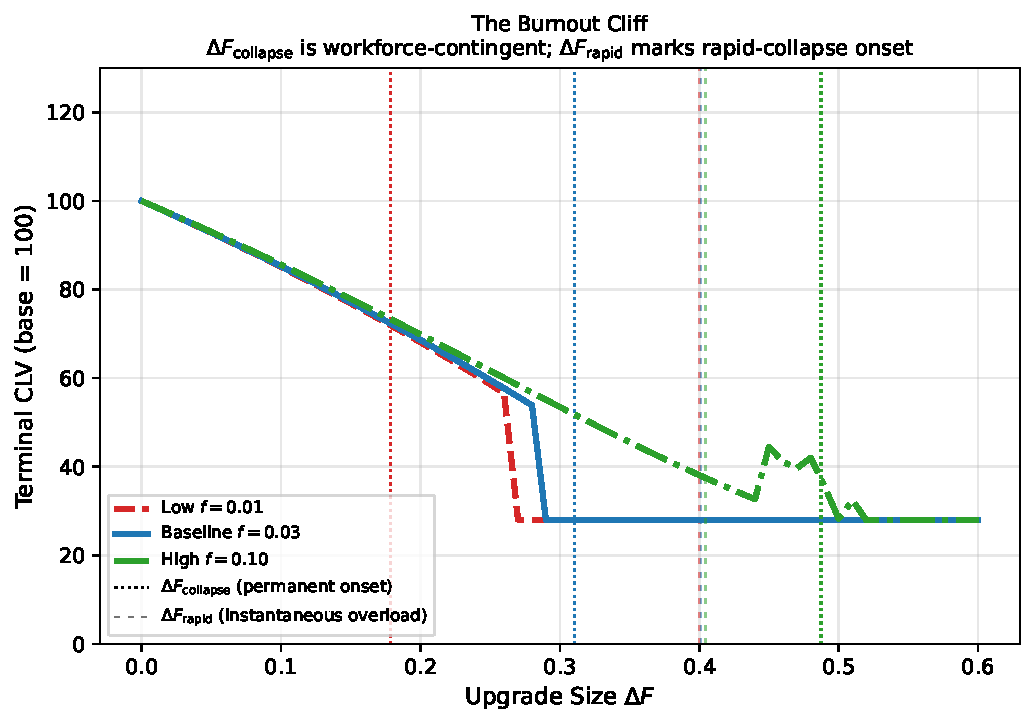
\includegraphics[width=0.75\textwidth]{fig5_burnout_cliff.pdf}}
{The Burnout Cliff. Terminal CLV (normalised to base$=100$ at $\Delta F=0$) as a function of upgrade size for three workforce-investment scenarios starting from their respective surplus equilibria at $F_0=0.80$. Dotted verticals mark the permanent-collapse onset $\Delta F_{\mathrm{collapse}} = F_{\mathrm{crit}}(f) - F_0$ (0.18, 0.31, and 0.49 for $f \in \{0.01, 0.03, 0.10\}$); dashed verticals mark the instantaneous-overload diagnostic $\Delta F_{\mathrm{rapid}} \approx 0.40$ (shown for $f \in \{0.01, 0.03\}$; for $f=0.10$, $\Delta F_{\mathrm{rapid}} < \Delta F_{\mathrm{collapse}}$ and no slow-collapse zone exists). The neglected-workforce firm ($f=0.01$, red) exhausts its safe zone at $\Delta F=0.18$; the invested firm ($f=0.10$, green) retains headroom to $\Delta F=0.49$. Workforce investment, not the current technology stock, sets the rollout speed limit.\label{fig:cliff}}
{}
\end{figure}


\section{Discussion}\label{sec:discussion}

\subsection{Contributions and Managerial Implications}\label{sec:disc:theory}

The three theorems together provide the formal micro-foundation that connects \citeauthor{ton2014good}'s (\citeyear{ton2014good}) four operational choices to each other through the dynamics of $\Keff$. Her prescription to ``operate with slack'' corresponds to the positive workforce investment rate $f$: operational slack keeps $W$ from depleting under moderate overload, and Theorem~\ref{thm:buffer} quantifies the CLV return to doing so. ``Standardise and empower'' corresponds to a lower overload sensitivity $\sigma$: well-designed processes reduce the per-unit depletion rate and enlarge the safe upgrade zone of Theorem~\ref{thm:cliff}. ``Offer less'' maps directly onto keeping $F$ below $F_{\mathrm{crit}}$: the model gives this demand-side lever a computable threshold rather than a qualitative prescription. ``Cross-train'' maps onto a higher complementarity parameter $p$: cross-trained workers raise effective capability $h(W)$ at any given engagement level, increasing the marginal return to both technology and workforce investment simultaneously (Proposition~\ref{prop:complementarity}). The model extends Oliva--Sterman with customer trust, a front-/back-stage domain split, and digital scaling: three extensions absent from the quality-erosion framework, now formalised in a single model that, to the best of our knowledge, provides the first dynamic formalisation of the service profit chain \citep{heskett1994putting} and Good Jobs Strategy \citep{ton2014good} with computable boundary conditions.

\medskip
\noindent\textbf{Managerial implications.} Four implications follow directly from the formal results. First, the maximum safe rollout speed is a workforce constraint (Theorem~\ref{thm:cliff}): before each deployment phase, the firm should verify that current workforce investment $f$ implies $\Delta F_{\mathrm{collapse}} = F_{\mathrm{crit}}(f) - F_0$ exceeds the planned upgrade size. Second, workforce well-being is a leading indicator of system health: $W$ reaches crisis levels roughly 11 months before trust does in the Scenario~A simulation, with the warning window ranging from 6 to 21 months depending on trust-update speed $\beta$ (EC Table~EC.4). Third, conventional workforce ROI calculations underestimate returns because the dominant capacity-multiplier channel is invisible in standard dashboards (Theorem~\ref{thm:buffer}; see §\ref{sec:analysis:buffer} for the mechanism-misattribution argument): when $p = 0$, equilibrium CLV is exactly invariant to $f$, confirming that the entire return to workforce investment flows through $h(W)$, not through operational sensing. Fourth, the more digital the firm becomes, the more it should invest in its people (Proposition~\ref{prop:complementarity}), a prescription at odds with prevailing practice: \citet{fisher2021staffing} document that profit-maximising staffing is considerably higher than what firms actually implement.

\subsection{Limitations and Directions for Future Research}\label{sec:disc:limits}

The three most consequential extensions are, in order of expected impact on the results: first, identification of $p$ from retailer panel data; second, a competitive multi-firm extension; and third, stochastic demand forcing. Several modelling choices bound the generality of the results and point toward these and other productive directions.

\paragraph{Exogenous front-stage capability and budget allocation.} The model treats $F$ as exogenous. As shown in \S\ref{sec:analysis:comp}, the Trap survives under budget-constrained joint choice of $F$ and $f$ (proof in EC~\S EC.1.7), but endogenising $F$ as a fourth state variable would enable analysis of optimal deployment sequencing. The current model also omits a direct $W \to D$ channel (unhappy employees visibly degrading the customer experience), making our results a conservative lower bound on the true workforce-capability complementarity.

\paragraph{The complementarity parameter $p$.} The parameter $p$ is the model's structurally most consequential assumption, driving all three theorems simultaneously (EC Table~EC.3). We view $p$ as the model's central testable prediction: in a store-level panel regression of CLV on $K$, $W$, and $K \times W$, the interaction coefficient estimates $p$ directly. Such estimation requires instrumental variables or quasi-experimental variation (e.g., technology rollouts) to address the simultaneity between $K$, $W$, and CLV, and represents the single most important empirical follow-up.

\paragraph{Model specification and stochastic extensions.} The power-law demand $D = (1+aT)F^b$ requires only convexity in $F$ for the Trap; replacing $h(W)$ with a concave form keeps the cross-partial positive but makes collapse irreversible (the linear form is conservative). The deterministic ODE omits demand shocks; adding diffusion terms would transform the Cliff into a probabilistic threshold. Empirically, the Front-Stage Trap predicts a negative three-way interaction between app deployment intensity, warehouse utilisation, and employee satisfaction in store-level CLV regressions.

\section{Conclusion}\label{sec:conclusion}

Standard operational dashboards measure the front-stage domain that invests in technology, not the back-stage workforce that fulfils the resulting demand and absorbs the consequences. This disconnect is not merely a measurement problem; it is a structural feature of omnichannel operations that makes cross-domain value destruction structurally predictable from two observable managerial choices: the workforce investment rate $f$ and the digitalisation level $F$. This paper provides the formal instrument for both.

Three results follow that, to our knowledge, no existing single formulation produces. The Front-Stage Trap (Theorem~\ref{thm:trap}): a computable digitalisation threshold $F_{\mathrm{crit}} \approx 1.11$ beyond which additional front-stage investment destroys CLV by overloading back-stage workers, a sign reversal impossible in single-domain models. The Good Jobs Buffer (Theorem~\ref{thm:buffer}): workforce investment raises CLV through a capacity-level channel confirmed exact by the $p{=}0$ counterfactual, which leaves CLV invariant to workforce spending and isolates the entire gain to service capacity. The Burnout Cliff (Theorem~\ref{thm:cliff}): the maximum safe upgrade size ranges from $\Delta F = 0.18$ for a workforce-neglecting firm to $\Delta F = 0.49$ for an investing firm, an approximately 172\% difference; the neglected firm retains approximately 37\% of the safe deployment headroom.

These results give operations teams two computable numbers standard dashboards do not report: a digitalisation ceiling ($F_{\mathrm{crit}}$) and a maximum safe rollout size ($\Delta F_{\mathrm{collapse}}$). Panel-data estimation of $p$ using technology rollout events as instruments, via the interaction coefficient in a store-level regression of CLV on $K$, $W$, and $K \times W$, is the single most important empirical follow-up. The broader implication extends beyond omnichannel retail: wherever automated front-stage processes generate demand on human back-stage operations, workforce investment is a structural requirement, not a social concession.


% ============================================================
% CODE AVAILABILITY
% ============================================================

\ACKNOWLEDGMENT{%
\textbf{Code Availability.}
All simulation code (Python, \texttt{wct\_simulation.py}) and figure-generation scripts used in this paper are available from the authors upon request and will be deposited in a permanent repository (OSF) upon acceptance.
The code is self-contained and requires only \texttt{numpy}, \texttt{scipy}, and \texttt{matplotlib}; all parameter values and study configurations are documented inline with references to the corresponding rows of Table~\ref{tab:params}.
}

% ============================================================
% BIBLIOGRAPHY
% PRODUCTION NOTE: The references "EC Table~EC.3" (tab:ec:sensitivity, sensitivity
% analysis table) and "EC Table~EC.4" (tab:ec:sensitivity2, supplementary sensitivity
% table) in the body are hardcoded cross-document references (lines ~204, ~228, ~463,
% ~469, ~506, ~514). If any EC table is added, removed, or reordered before final
% production, these five body locations must be updated manually.
% ============================================================

%\bibliographystyle{informs2014}
%\bibliography{wct_refs}

\begin{thebibliography}{99}

\bibitem[Acimovic and Graves(2015)]{acimovic2015fulfillment}
Acimovic J, Graves SC (2015) Making better fulfillment decisions on the fly in an online retail environment.
\textit{Manufacturing \& Service Operations Management} 17(1):34--51.

\bibitem[Argote and Epple(1990)]{argote1990learning}
Argote L, Epple D (1990) Learning curves in manufacturing.
\textit{Science} 247(4945):920--924.

\bibitem[Bainbridge(1983)]{bainbridge1983ironies}
Bainbridge L (1983) Ironies of automation.
\textit{Automatica} 19(6):775--779.

\bibitem[Bakker and Demerouti(2007)]{bakker2007job}
Bakker AB, Demerouti E (2007) The Job Demands-Resources model: State of the art.
\textit{Journal of Managerial Psychology} 22(3):309--328.

\bibitem[Baumeister et~al.(2001)]{baumeister2001bad}
Baumeister RF, Bratslavsky E, Finkenauer C, Vohs KD (2001) Bad is stronger than good.
\textit{Review of General Psychology} 5(4):323--370.

\bibitem[Bell et~al.(2018)]{bell2018inventory}
Bell DR, Gallino S, Moreno A (2018) Offline showrooms in omnichannel retail: Demand and operational benefits.
\textit{Management Science} 64(4):1629--1651.

\bibitem[Bijmolt et~al.(2021)]{bijmolt2021challenges}
Bijmolt THA, Broekhuis M, de~Leeuw S, Hirche C, Rooderkerk RP, Sousa R, Zhu SX (2021) Challenges at the marketing-operations interface in omni-channel retail environments.
\textit{Journal of Business Research} 122:864--874.

\bibitem[Aral et~al.(2012)]{aral2012three}
Aral S, Brynjolfsson E, Wu L (2012) Three-way complementarities: Performance pay, human resource analytics, and information technology.
\textit{Management Science} 58(5):913--931.

\bibitem[Corbett(2024)]{corbett2024wellbeing}
Corbett CJ (2024) OM Forum: The operations of well-being: An operational take on happiness, equity, and sustainability.
\textit{Manufacturing \& Service Operations Management} 26(2):409--430.

\bibitem[Dub{\'{e}} et~al.(2020)]{dube2020minimum}
Dub{\'{e}} A, Reich A, Shierholz H, West M (2020) Minimum wage shocks, employment flows and labor market frictions.
\textit{Journal of Labor Economics} 38(4):1009--1052.

\bibitem[Demerouti et~al.(2001)]{demerouti2001job}
Demerouti E, Bakker AB, Nachreiner F, Schaufeli WB (2001) The Job Demands-Resources model of burnout.
\textit{Journal of Applied Psychology} 86(3):499--512.

\bibitem[Filippov(1988)]{filippov1988differential}
Filippov AF (1988) \textit{Differential Equations with Discontinuous Righthand Sides}.
Dordrecht: Kluwer Academic Publishers.

\bibitem[Fisher et~al.(2021)]{fisher2021staffing}
Fisher ML, Gallino S, Netessine S (2021) Setting retail staffing levels: A methodology validated with implementation.
\textit{Manufacturing \& Service Operations Management} 23(6):1562--1579.

\bibitem[Gans and Goldfarb(2026)]{gans2026oring}
Gans JS, Goldfarb A (2026) O-ring automation.
NBER Working Paper No.\ 34639. National Bureau of Economic Research, Cambridge, MA.

\bibitem[Gupta et~al.(2004)]{gupta2004valuing}
Gupta S, Lehmann DR, Stuart JA (2004) Valuing customers.
\textit{Journal of Marketing Research} 41(1):7--18.

\bibitem[Heskett et~al.(1994)]{heskett1994putting}
Heskett JL, Jones TO, Loveman GW, Sasser Jr WE, Schlesinger LA (1994) Putting the service-profit chain to work.
\textit{Harvard Business Review} 72(2):164--174.


\bibitem[H{\"u}bner et~al.(2021)]{hubner2021digitalization}
H{\"u}bner A, Amorim P, Fransoo JC, Honhon D, Kuhn H, Martinez~de~Albeniz V, Robb D (2021) Digitalization and omnichannel retailing: Innovative OR approaches for retail operations.
\textit{European Journal of Operational Research} 294(3):817--819.

\bibitem[KC and Terwiesch(2009)]{kc2009impact}
KC D, Terwiesch C (2009) Impact of workload on service time and patient safety: An econometric analysis of hospital operations.
\textit{Management Science} 55(9):1486--1498.

\bibitem[Kesavan et~al.(2022)]{kesavan2022doing}
Kesavan S, Lambert SJ, Williams JC, Pendem PK (2022) Doing well by doing good: Improving retail store performance with responsible scheduling practices at the Gap, Inc.
\textit{Management Science} 68(11):7818--7836.

\bibitem[Kremer(1993)]{kremer1993oring}
Kremer M (1993) The O-ring theory of economic development.
\textit{Quarterly Journal of Economics} 108(3):551--575.

\bibitem[Krusell et~al.(2000)]{krusell2000capital}
Krusell P, Ohanian LE, R\'ios-Rull JV, Violante GL (2000) Capital-skill complementarity and inequality: A macroeconomic analysis.
\textit{Econometrica} 68(5):1029--1053.

\bibitem[Martinez-Moyano et~al.(2014)]{martinez2014drift}
Martinez-Moyano IJ, McCaffrey DP, Oliva R (2014) Drift and adjustment in organizational rule compliance.
\textit{Organization Science} 25(1):44--65.

\bibitem[Mas and Moretti(2009)]{mas2009peers}
Mas A, Moretti E (2009) Peers at work.
\textit{American Economic Review} 99(1):112--145.

\bibitem[McKnight et~al.(2002)]{mcknight2002developing}
McKnight DH, Choudhury V, Kacmar C (2002) Developing and validating trust measures for e-commerce: An integrative typology.
\textit{Information Systems Research} 13(3):334--359.

\bibitem[Milgrom and Roberts(1990)]{milgrom1990economics}
Milgrom P, Roberts J (1990) The economics of modern manufacturing: Technology, strategy, and organization.
\textit{American Economic Review} 80(3):511--528.

\bibitem[Mittal et~al.(1998)]{mittal1998asymmetric}
Mittal V, Ross WT, Baldasare PM (1998) The asymmetric impact of negative and positive attribute-level performance on overall satisfaction and repurchase intentions.
\textit{Journal of Marketing} 62(1):33--47.

\bibitem[Oliva and Sterman(2001)]{oliva2001cutting}
Oliva R, Sterman JD (2001) Cutting corners and working overtime: Quality erosion in the service industry.
\textit{Management Science} 47(7):894--914.

\bibitem[Oliva et~al.(2003)]{oliva2003limits}
Oliva R, Sterman JD, Giese M (2003) Limits to growth in the new economy: Exploring the `get big fast' strategy in e-commerce.
\textit{System Dynamics Review} 19(2):83--117.

\bibitem[Rahmandad and Repenning(2016)]{rahmandad2016capability}
Rahmandad H, Repenning N (2016) Capability erosion dynamics.
\textit{Strategic Management Journal} 37(4):649--672.

\bibitem[Repenning and Sterman(2001)]{repenning2001nobody}
Repenning NP, Sterman JD (2001) Nobody ever gets credit for fixing problems that never happened.
\textit{California Management Review} 43(4):64--88.

\bibitem[Saghiri et~al.(2017)]{saghiri2017toward}
Saghiri S, Wilding R, Mena C, Bourlakis M (2017) Toward a three-dimensional framework for omni-channel.
\textit{Journal of Business Research} 77:53--67.

\bibitem[Sirdeshmukh et~al.(2002)]{sirdeshmukh2002consumer}
Sirdeshmukh D, Singh J, Sabol B (2002) Consumer trust, value, and loyalty in relational exchanges.
\textit{Journal of Marketing} 66(1):15--37.

\bibitem[Sterman(2000)]{sterman2000business}
Sterman JD (2000) \textit{Business Dynamics: Systems Thinking and Modeling for a Complex World}.
Boston: Irwin/McGraw-Hill.

\bibitem[Ton(2014)]{ton2014good}
Ton Z (2014) \textit{The Good Jobs Strategy: How the Smartest Companies Invest in Employees to Lower Costs and Boost Profits}.
New York: Houghton Mifflin Harcourt.

\bibitem[Tucker(2007)]{tucker2007operational}
Tucker AL (2007) An empirical study of system improvement by frontline employees in hospital units.
\textit{Manufacturing \& Service Operations Management} 9(4):492--505.

\end{thebibliography}

\end{document}